\chapter{Speicher}

\section{Moderne File Systeme}

\subsection{Sie wissen was ein modernes Filesystem leisten muss.}

Ein modernes Filesystem sollte folgende Anforderungen erfüllen:
\begin{itemize}
	\item grosse Adressierbarkeit
	\item Volume Manager eingebaut
	\item umfangreiche Funktionalitäten
	\item immer konsistent und integer
	\item kein fsck mehr nötig nach Absturz
	\item kann mit \emph{silent corruption} umgehen (unabsichtliche Änderungen von Bits)
\end{itemize}
Ein schon etwas in die Jahre gekommenes Filesystem ist das Unix File System (UFS). Im UFS werden Daten in Blöcken abgelegt und alle Informationen zu einer Datei sind in sogenannten \texttt{inodes} abgelegt. Das Dateisystem ist hierarchisch aufgebaut wobei die Hierarchiestufen Verzeichnisse, Dateien oder Laufwerke sein können. UFS hat ein paar Nachteile s können in der aktuellen Version nur 1 TB adressiert werden und auch fsck muss nach einem Absturz ausgeführt werden.

Ein Beispiel für ein modernes Filesystem ist ZFS welches von Sun Microsystems entwickelt wurde. Eine gute Übersicht bietet dieser Artikel: \href{http://www.admin-magazin.de/Online-Artikel/ZFS-Snapshots-RAID-und-Datensicherheit}{http://www.admin-magazin.de/Online-Artikel/ZFS-Snapshots-RAID-und-Datensicherheit}

\subsection{Sie wissen wie ein modernes Filesystem aufgebaut ist.}

\subsubsection{Volumes vs. Pooled Storage}

Bei traditionellen Filesystemen war ein Filesystem für eine physikalische Partition zuständig. Wollte man mehrere physikalische Partitionen zu einer logischen Partition zusammenfassen musste man zusätzlich einen Logical Volume Manager installieren. Durch logische Volumen kann man z.B. Speicherplatz von zwei Festplatten zusammenfassen oder ein Volume spiegeln.
ZFS fasst diese Funktionen zusammen indem die physischen Datenträger (alles vom Floppy bis zur SSD) in einem Pool zusammengefasst werden. Aus diesem Pool können das beliebig viele logische Partitionen mit eigenem Dateisystem erstellt werden. Die logischen Partitionen können dynamisch wachsen oder durch den Admin eingeschränkt werden.
Klassische Dateisysteme abstrahieren zwar die Festplattenlogik, müssen dadurch aber komplizierte Strukturen erstellen um die Dateien abzuspeichern (kostet Zeit). ZFS verwendet zur Speicherung von Dateien und Metadaten ZFS-Objekte welche die DMU (Data Management Unit) zur Verfügung stellt. Wird nun eine Schreiboperation vom Betriebssystem ausgelöst, startet die DMU eine Transaktion. Gleichzeitig abschliessende Transaktionen werden zu Transaktionsgruppen gesammelt und dem SPA (Storage Pool Allocator) übergeben, welcher sie auf die physikalischen Platten schreibt.

\subsubsection{Konsistenz}

Nach einem Systemzusammenbruch kann das Filesystem in einem inkonsistenten Zustand sein, insbesondere wenn Blöcke für die Dateiverwaltung nicht korrekt auf die Festplatte geschrieben wurden. Mittels \texttt{fsck} wird ein Konsistenztest auf File- und Blockebene durchgeführt (Blöcke weder frei noch File zugeordnet, Block tritt mehrfach auf usw.). \texttt{fsck} kann bei grossen Dateisystemen sehr lange dauern und man möchte ständig wissen ob die Daten korrupt sind. Um jederzeit konsistent zu sein können Dateien auf zwei Arten geschrieben werden:
\begin{description}
	\item[CoW (Copy On Write):] Die alten Daten werden in einen neuen Speicherblock kopiert. Die Daten im alten Speicherblock werden überschrieben mit den neuen Daten.
	\item[RoW (Redirect On Write):] Neue Schreibanfrage möchte die Daten in den alten Block schreiben. Diese werden aber in einen neuen Block geschrieben (redirect). Der Originalblock enthält alte Daten.
\end{description}
ZFS verwendet CoW obwohl es eher ein RoW ist. Abbildung \ref{fig:write-file-zfs} zeigt wie eine Datei im ZFS geschrieben wird. Nachfolgend sind die einzelnen Schritte beschrieben:
\begin{enumerate}
	\item Man geht vom konsistenten Zustand aus, bei dem das Filesystem mit den blauen Blöcken vollständig in Ordnung ist. Die Daten liegen dabei nur in den Blättern des Baumes. Die inneren Knoten des Baumes enthalten lediglich Zeiger und keine sonstigen Daten. Die separat gespeicherte Wurzel des Baumes heisst bei ZFS Überblock.
	\item Nun sind ein paar Dateien zu schreiben. ZFS sucht dafür freie, momentan unbenutzte Blöcke (im Bild sind diese Blöcke grün hervorgehoben), es überschreibt niemals belegte. Ausserdem achtet es darauf, dass die Blöcke möglichst beieinander liegen, um effizient schreiben zu können. Noch gelangen die Daten aber nicht auf die Platte, weil sonst die Transaktion nicht mehr rückgängig zu machen wäre.
	\item Irgendwann schliesst das Betriebssystem die Transaktion ab (commit). Dazu ist der Baum bis zur Wurzel zu aktualisieren. Der linke Block in der mittleren Ebene erhält die Zeiger auf die beiden neuen Datenblöcke. Der linke Block auf der Ebene darüber erhält links den Zeiger auf den eben modifizierten Block, und rechts wird der unveränderte Teil eingetragen. Dieser Schritt fasst in der Regel mehrere Schreibvorgänge in einer so genannten Transaktionsgruppe zusammen.
	\item Nun ist alles vorbereitet, um die Transaktion endgültig zu beenden. Dazu schreibt ZFS den Überblock (im Bild: kleines Quadrat). Ist der neue Überblock erzeugt, sind die eben erstellten Blöcke im Filesystem aktiv. Bricht das System aus irgendeinem Grund ab (»halt«-Kommando an der Konsole, Systemabsturz, Stromausfall, ...), dann existiert noch der alte Überblock und damit der alte Zustand in den blauen Blöcken, denn das Filesystem beschrieb lediglich Blöcke, die im Ausgangszustand (blau) unbenutzt waren.
\end{enumerate}
\begin{figure}
\centering
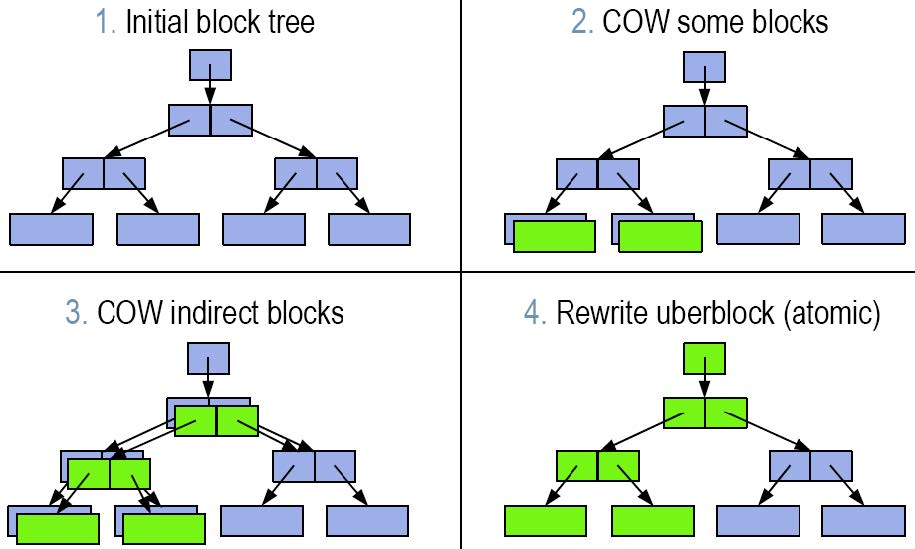
\includegraphics[width=0.7\linewidth]{fig/write-file-zfs}
\caption{Datei schreiben in ZFS}
\label{fig:write-file-zfs}
\end{figure}
Wenn beim schreiben des Überblocks etwas schiefgeht hat ZFS auch diverse Mechanismen auf Lager um ihn wiederherzustellen.

\subsubsection{Snapshots}

Snapshots bezeichnen eine Kopie eines Filesystems zu einem bestimmten Zeitpunkt, die nicht mehr veränderlich ist. In ZFS lässt sich ein solcher Snapshot sehr einfach herstellen: Man merkt sich lediglich den Zeiger auf den Wurzelknoten des Filesystems und hat damit den Snapshot ohne grossen Aufwand bereits realisiert. Da bei Änderungen nie Datenblöcke überschrieben werden, kann der Snapshot weiterhin die alten Datenblöcke referenzieren. Wird eine Datei verändert und möchte man diese in den Snapshot übernehmen muss lediglich die Referenz geändert werden (Abbildung \ref{fig:snapshot}).

\begin{figure}
\centering
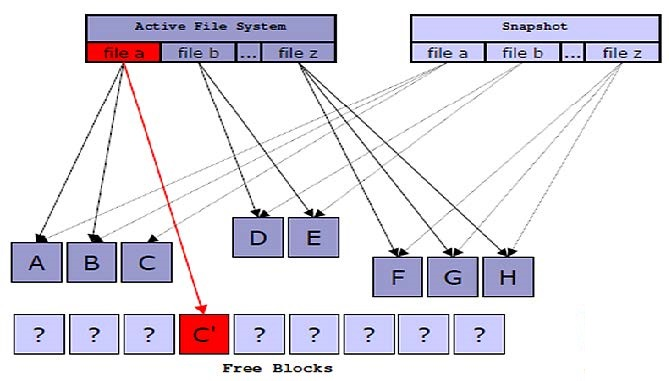
\includegraphics[width=0.7\linewidth]{fig/snapshot}
\caption{Snapshot}
\label{fig:snapshot}
\end{figure}

\subsubsection{Selbstheilung}

Herkömmliche Filesysteme setzen auf Sektorprüfsummen und RAID um Datenverlust zu verhindern. Diese Techniken erkennen aber eine ganze Reihe von Fehlern nicht. ZFS kann Daten selbstständig redundant speichern (RAID 1) und beherrscht auch eine verbesserte RAID 5-Variante welche sich RAID z nennt. Zusätzlich zu diesen bekannten Techniken kann sich ZFS selbst heilen. Wenn ein herkömmliches Filesystem einen defekten Block liest bleibt das unbemerkt, auch wenn eine Spiegelung des defekten Blockes vorhanden ist. Der defekte Block wird dann vom User Prozess verarbeitet, was zu Systemabstürzen führen kann. ZFS erkennt solche defekten Blöcke zur Laufzeit mittels Prüfsumme und ersetzt den defekten Block mit seiner Spiegelung auf einem anderem Device. Zusätzlich kann ZFS den defekten Block auch reparieren. Dieser Vorgang muss jedoch manuell ausgelöst werden.

\subsection{Sie wissen wie der Kern und das File System zusammenarbeiten.}

\subsubsection{Buffer Cache}

Wenn ein Prozess auf Datenblöcke eines Files zugreifen will, so bringt der Kern diese Blöcke in den Hauptspeicher, ändert diese nach Bedarf und macht danach eine Anfrage diese im File System zu speichern (z.B. \texttt{cp fileone.c filetwo.c}). Um den Durchsatz zu erhöhen richtet der Kern beim Systemstart einen sogenannten Buffer Cache ein. Der Buffer Cache ist eine Softwarestruktur welche den Durchsatz drastisch erhöhen kann. Der Datentransfer zwischen dem Buffer Cache (Kern-Raum) und dem User Prozess-Raum wird immer über DMA (Direct Memory Access) gemacht, weil so keine Prozessor-Zyklen verbraucht werden.
Ein Buffer besteht aus zwei Teilen:
\begin{description}
	\item[Memory Array:] Speicherblöcke
	\item[Buffer Header:] Kopf eines Speicherblockes mit Metadaten
\end{description} 
Der Buffer Header hat ca. 20 Einträge. Die folgenden Einträge kennzeichnen den Datenblock im Memory Array:
\begin{description}
	\item[Device Nummer:] ID vom angeschlossenen Gerät (Harddisk, USB-Stick usw.)
	\item[Block Nummer:] ID von Daten auf der Disk
	\item[Status vom Block:] Buffer gesperrt, Buffer enthält gültige Daten, verzögertes Schreiben, Kern liest/schreibt Inhalt, Prozess wartet bis Buffer frei wird
\end{description}
Der Kern identifiziert den Bufferinhalt indem er die Device- und Blocknummer überprüft. Der Kern unterhält zwei doppelt verknüpfte Listen. Eine \emph{Freie Liste} in welcher alle freien Buffer eingetragen sind und eine Hash-Queue (Hash über Device- und Blocknummer) welche verwendet wird um auf einen Disk Block zuzugreifen.

%TODO Buffer Szenarien (bin nicht drausgekommen).

\subsubsection{Virtual File System (VFS)}

Das VFS ist eine Abstraktion des zugrundeliegenden Filesystems und bietet eine einheitliche Schnittstelle für die Dateimanipulation einem User Prozess an. Die Schnittstelle kann von einem User Prozess im POSIX Format angesprochen werden (z.B. \texttt{open( „/usr/include/unistd.h“, O\_RDONLY)}) Das VFS setzt voraus dass ein File einen einzigartigen Namen und einen Benutzer hat. Für jedes spezifische Filesystem wird ein Mapping Modul bereitgestellt welches das reelle Filesystem auf das virtuelle Filesystem transformiert. Auf der Abbildung \ref{fig:virtual-file-system} ist dieses Mapping im Detail abgebildet.

\begin{figure}
\centering
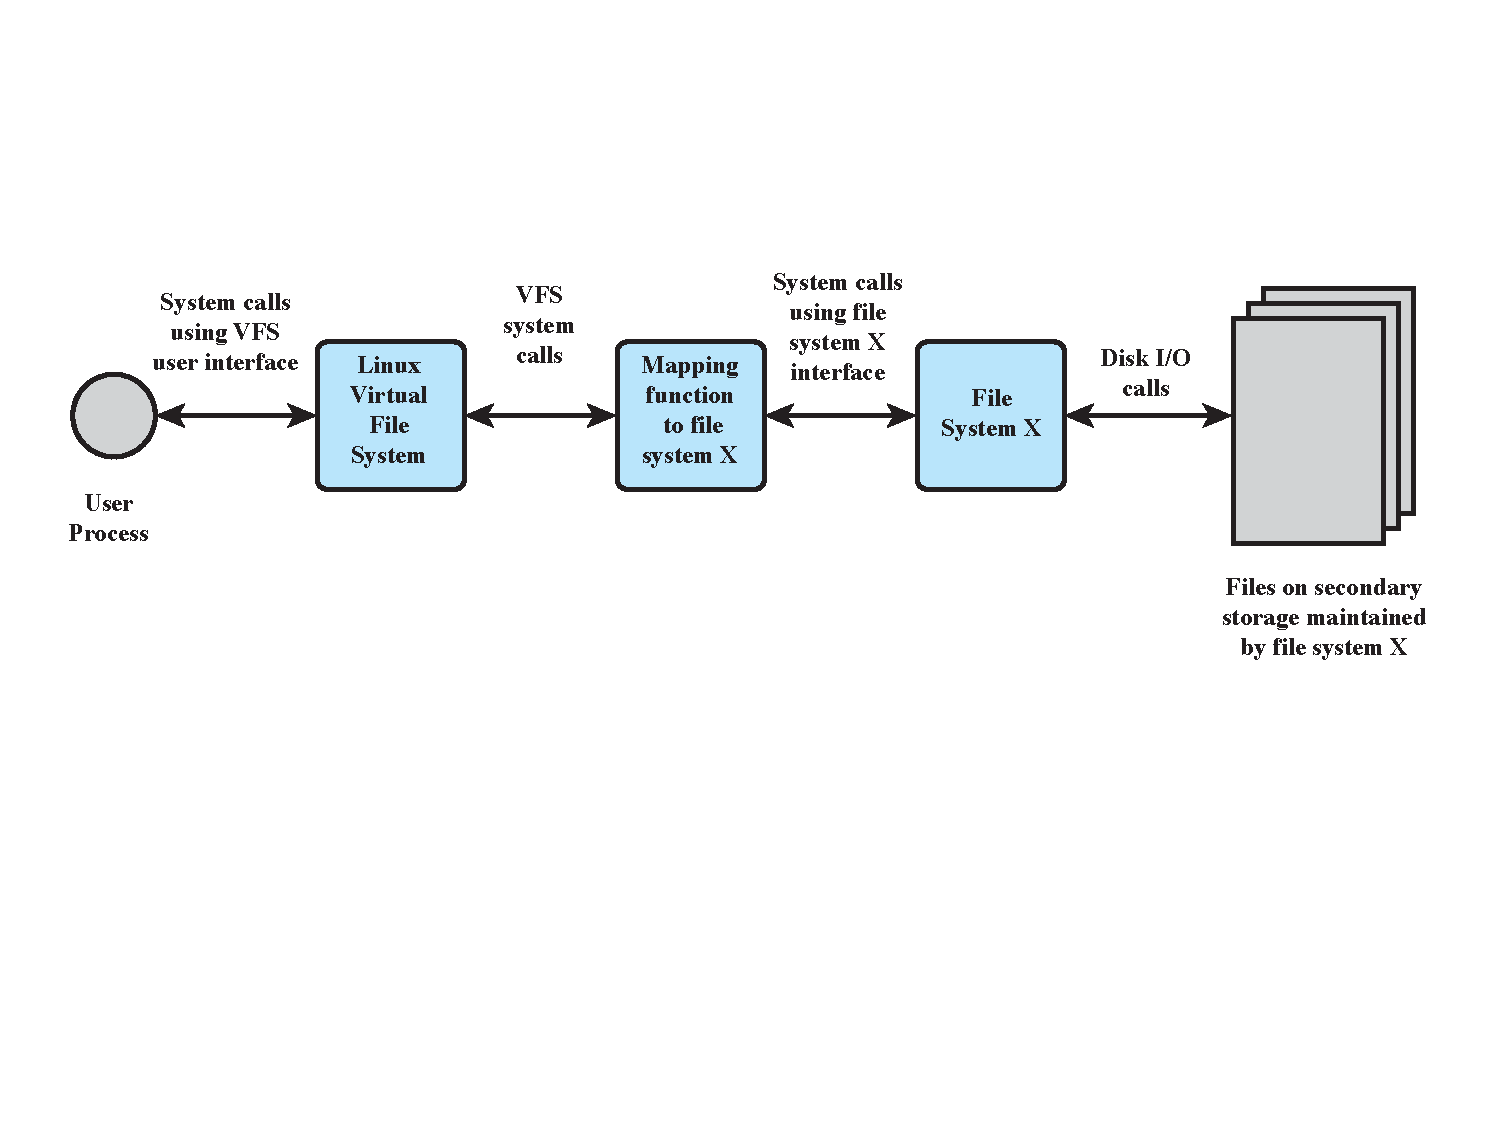
\includegraphics[width=0.7\linewidth]{fig/virtual-file-system}
\caption{Virtual File System}
\label{fig:virtual-file-system}
\end{figure}

\subsection{Sie kennen die internen Strukturen eines Filesystems.}

Das ZFS ist in einer Baumstruktur (Merkle Tree) aufgebaut. Der Wurzelknoten wird \emph{Uberblock} genannt. Die Knoten zwischen dem \emph{Uberblock} und den Blättern enthalten Block Pointers. Block Pointer enthalten \emph{Data Virtual Addresses} zu anderen Blöcken und zusätzlich auch den Hash von seinen Kind Knoten. Die Blätter des Baumes enthalten dann die eigentlichen Daten.

\section{Speichernetze \& Protokolle}